% GAL1897 W01 -- source-faithful preliminary matter
% Assigned source: physical PDF pages 001--023 / JP2 leaves L0000--L0022.
% Protected read-only next neighbor: PDF 024 / L0023 (Introduction, printed folio v).
% UTF-8 LaTeX fragment. Requires graphicx. The page-disposition CSV is authoritative
% for excluded platform/library matter and for inspected blank topology.

\providecommand{\GalExcludedSourcePage}[4]{}%
\providecommand{\GalBlankTopologyPage}[4]{}%
\providecommand{\GalSourcePageBegin}[2]{\clearpage\thispagestyle{empty}}%
\providecommand{\GalSourcePageEnd}{\par}%
\providecommand{\GalWitnessNote}[3]{%
  \par\smallskip\begingroup\footnotesize\noindent\textbf{#2.} #3\GalEditorialReference{#1}\endgroup\smallskip}%
\providecommand{\GalUnresolvedSourcePage}[4]{#4}%

% PDF 001 / L0000 -- modern Google platform notice; intentionally not typeset.
\GalExcludedSourcePage{001}{L0000}{platform_boilerplate}{Modern Google digitization and usage notice.}
% PDF 002 / L0001 -- Harvard library bookplate/shelfmark; intentionally not typeset.
\GalExcludedSourcePage{002}{L0001}{library_accession}{Harvard College Library bookplate and shelfmark.}
% PDF 003--006 / L0002--L0005 -- inspected blank topology.
\GalBlankTopologyPage{003}{L0002}{blank}{No historical letterpress or image.}
\GalBlankTopologyPage{004}{L0003}{blank}{No historical letterpress or image.}
\GalBlankTopologyPage{005}{L0004}{blank}{No historical letterpress or image.}
\GalBlankTopologyPage{006}{L0005}{blank}{No historical letterpress or image.}

% PDF 007 / L0006 -- full title/wrapper page.
\GalSourcePageBegin{007}{L0006}
% ENSEG:W01:PDF007:0001
\begin{center}
\vspace*{0.012\textheight}
{\fontsize{30}{34}\selectfont\bfseries MATHEMATICAL\par}
\vspace{0.55em}
{\large\bfseries WORKS\par}
\vspace{0.75em}
{\fontsize{23}{27}\selectfont\bfseries OF ÉVARISTE GALOIS,\par}
\vspace{0.95em}
{\small\bfseries PUBLISHED\par}
\vspace{0.45em}
{\small\bfseries UNDER THE AUSPICES OF THE MATHEMATICAL SOCIETY OF FRANCE,\par}
\vspace{0.95em}
{\Large\bfseries WITH AN INTRODUCTION\par}
\vspace{0.40em}
{\small\bfseries BY\par}
\vspace{0.35em}
{\Large\bfseries M. ÉMILE PICARD,\par}
{\small\bfseries MEMBER OF THE INSTITUTE OF FRANCE.\par}
\vspace{0.80em}

\includegraphics[height=0.105\textheight,keepaspectratio]{figures/PDF007_L0006_PUBLISHER_DEVICE.png}\par
\vspace{0.60em}
{\Large\bfseries PARIS,\par}
\vspace{0.30em}
{\small\bfseries GAUTHIER-VILLARS ET FILS, PRINTERS AND BOOKSELLERS\par}
{\footnotesize\bfseries TO THE BUREAU OF LONGITUDES AND THE ÉCOLE POLYTECHNIQUE,\par}
{\small\bfseries 55, Quai des Grands-Augustins.\par}
\vspace{0.35em}
{\Large\bfseries 1897\par}
{\small\bfseries (All rights reserved.)\par}
\end{center}
  \GalWitnessNote{W01-U003}{Marks beneath the title remain unread}{Two handwritten strokes appear beneath ``GALOIS'' in the 1897 image. The publisher's device is reproduced as an image, and its ribbon legend is not expanded into uncertain text.}
\GalSourcePageEnd

% PDF 008--011 / L0007--L0010 -- inspected blank topology.
\GalBlankTopologyPage{008}{L0007}{blank}{No historical letterpress or image.}
\GalBlankTopologyPage{009}{L0008}{blank}{No historical letterpress or image.}
\GalBlankTopologyPage{010}{L0009}{blank}{No historical letterpress or image.}
\GalBlankTopologyPage{011}{L0010}{blank}{No historical letterpress or image.}

% PDF 012 / L0011 -- half-title.
\GalSourcePageBegin{012}{L0011}
% ENSEG:W01:PDF012:0002
\begin{center}
\vspace*{0.38\textheight}
{\fontsize{32}{38}\selectfont\bfseries MATHEMATICAL\par}
\vspace{1.4em}
{\large\bfseries WORKS\par}
\vspace{1.6em}
{\fontsize{25}{30}\selectfont\bfseries OF ÉVARISTE GALOIS.\par}
\end{center}
\GalSourcePageEnd

% PDF 013 / L0012 -- Harvard bequest label and manuscript shelfmarks; intentionally not typeset.
\GalExcludedSourcePage{013}{L0012}{library_accession}{Harvard College Library bequest label and shelfmarks.}
% PDF 014 / L0013 -- inspected blank topology.
\GalBlankTopologyPage{014}{L0013}{blank}{No historical letterpress or image.}

% PDF 015 / L0014 -- printer imprint.
\GalSourcePageBegin{015}{L0014}
% ENSEG:W01:PDF015:0003
\begin{center}
\vspace*{0.42\textheight}
\rule{0.22\textwidth}{0.4pt}\par
\vspace{1.0em}
{\normalsize\bfseries Paris. --- Printing House of GAUTHIER-VILLARS ET FILS,\par}
{\normalsize\bfseries 55, quai des Grands-Augustins.\par}
\vspace{1.0em}
\rule{0.22\textwidth}{0.4pt}\par
\end{center}
\GalSourcePageEnd

% PDF 016--018 / L0015--L0017 -- inspected blank topology.
\GalBlankTopologyPage{016}{L0015}{blank}{No historical letterpress or image.}
\GalBlankTopologyPage{017}{L0016}{blank}{No historical letterpress or image.}
\GalBlankTopologyPage{018}{L0017}{blank}{No historical letterpress or image.}

% PDF 019 / L0018 -- portrait plate and caption.
\GalSourcePageBegin{019}{L0018}
% ENSEG:W01:PDF019:0004
\begin{center}
\vspace*{0.05\textheight}
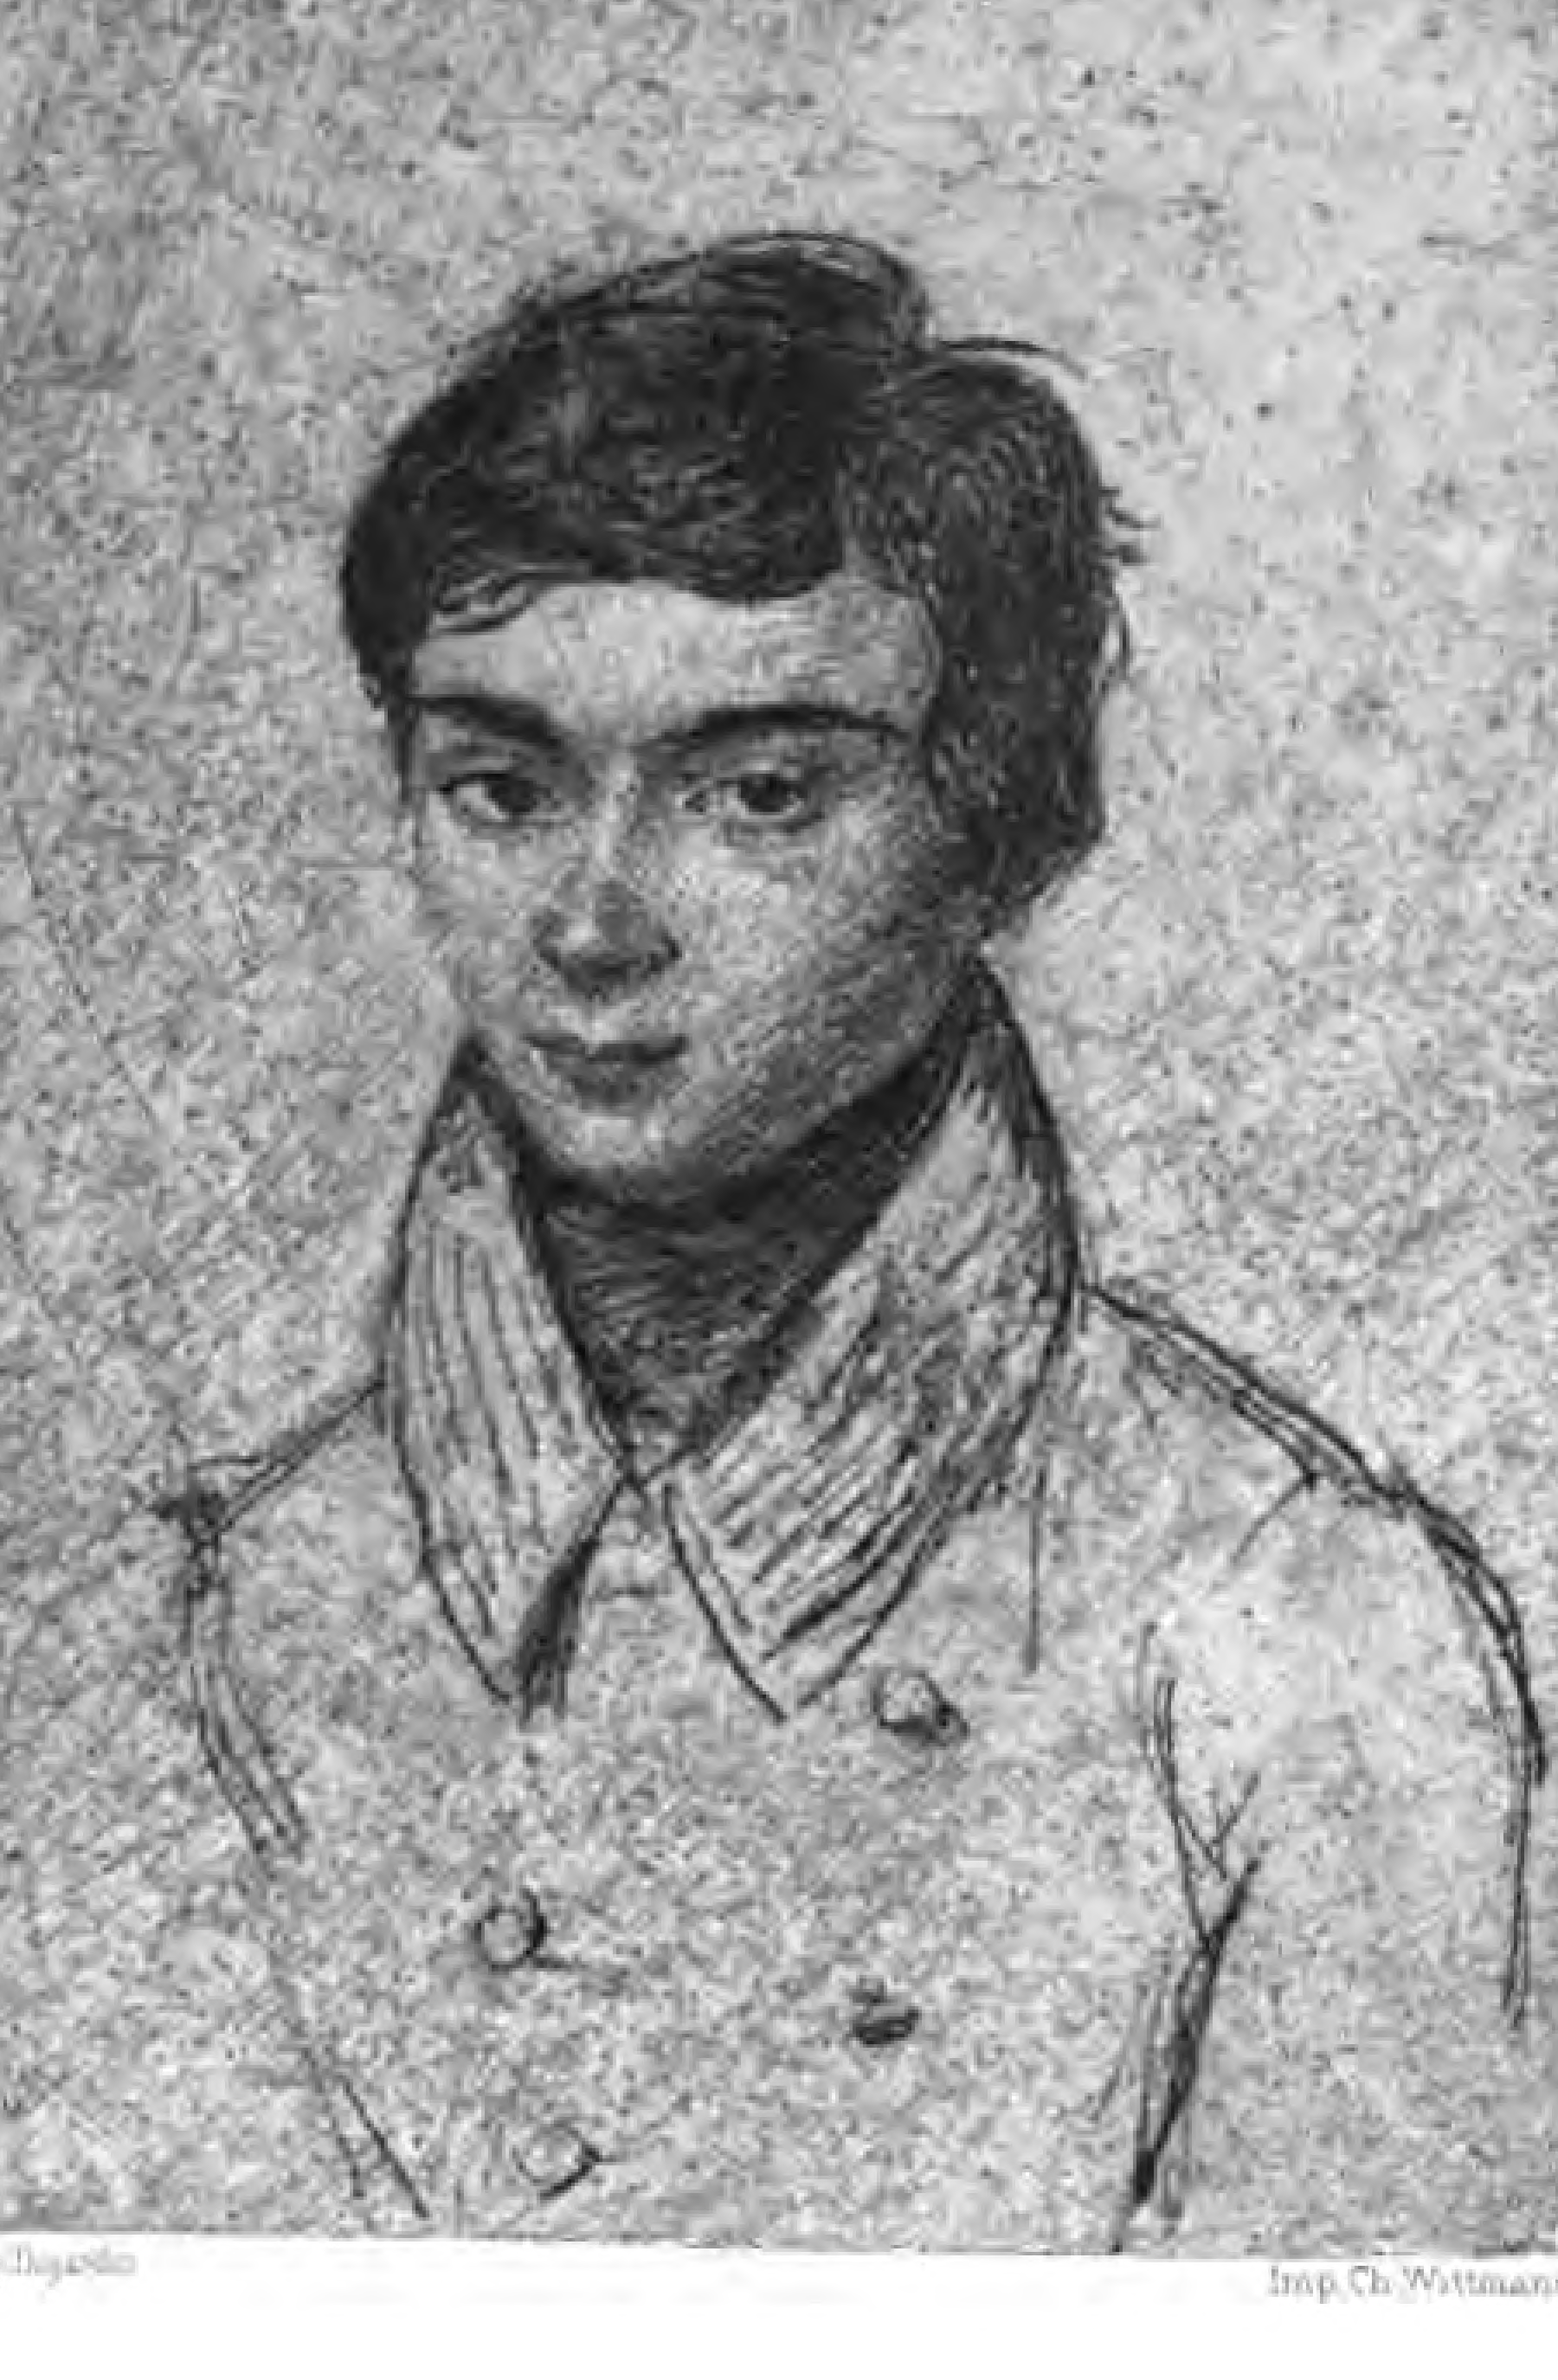
\includegraphics[height=0.61\textheight,keepaspectratio]{figures/PDF019_L0018_PORTRAIT_PLATE.png}\par
\vspace{1.0em}
{\Large E. GALOIS\par}
\end{center}
\GalWitnessNote{W01-U001}{The portrait signature is too faint to read}{The lower-right plate imprint reads ``Imp. Ch. Wittmann.'' The faint signature at lower left cannot be read securely and is therefore preserved only in the reproduced image.}
\GalSourcePageEnd

% PDF 020 / L0019 -- inspected blank topology.
\GalBlankTopologyPage{020}{L0019}{blank}{No historical letterpress or image.}

% PDF 021 / L0020 -- severely degraded second portrait plate; relation to PDF 019 unresolved.
\GalUnresolvedSourcePage{021}{L0020}{apparent_duplicate_portrait}{%
  \GalSourcePageBegin{021}{L0020}
  % ENSEG:W01:PDF021:0005
  \begin{center}
  \vspace*{0.05\textheight}
  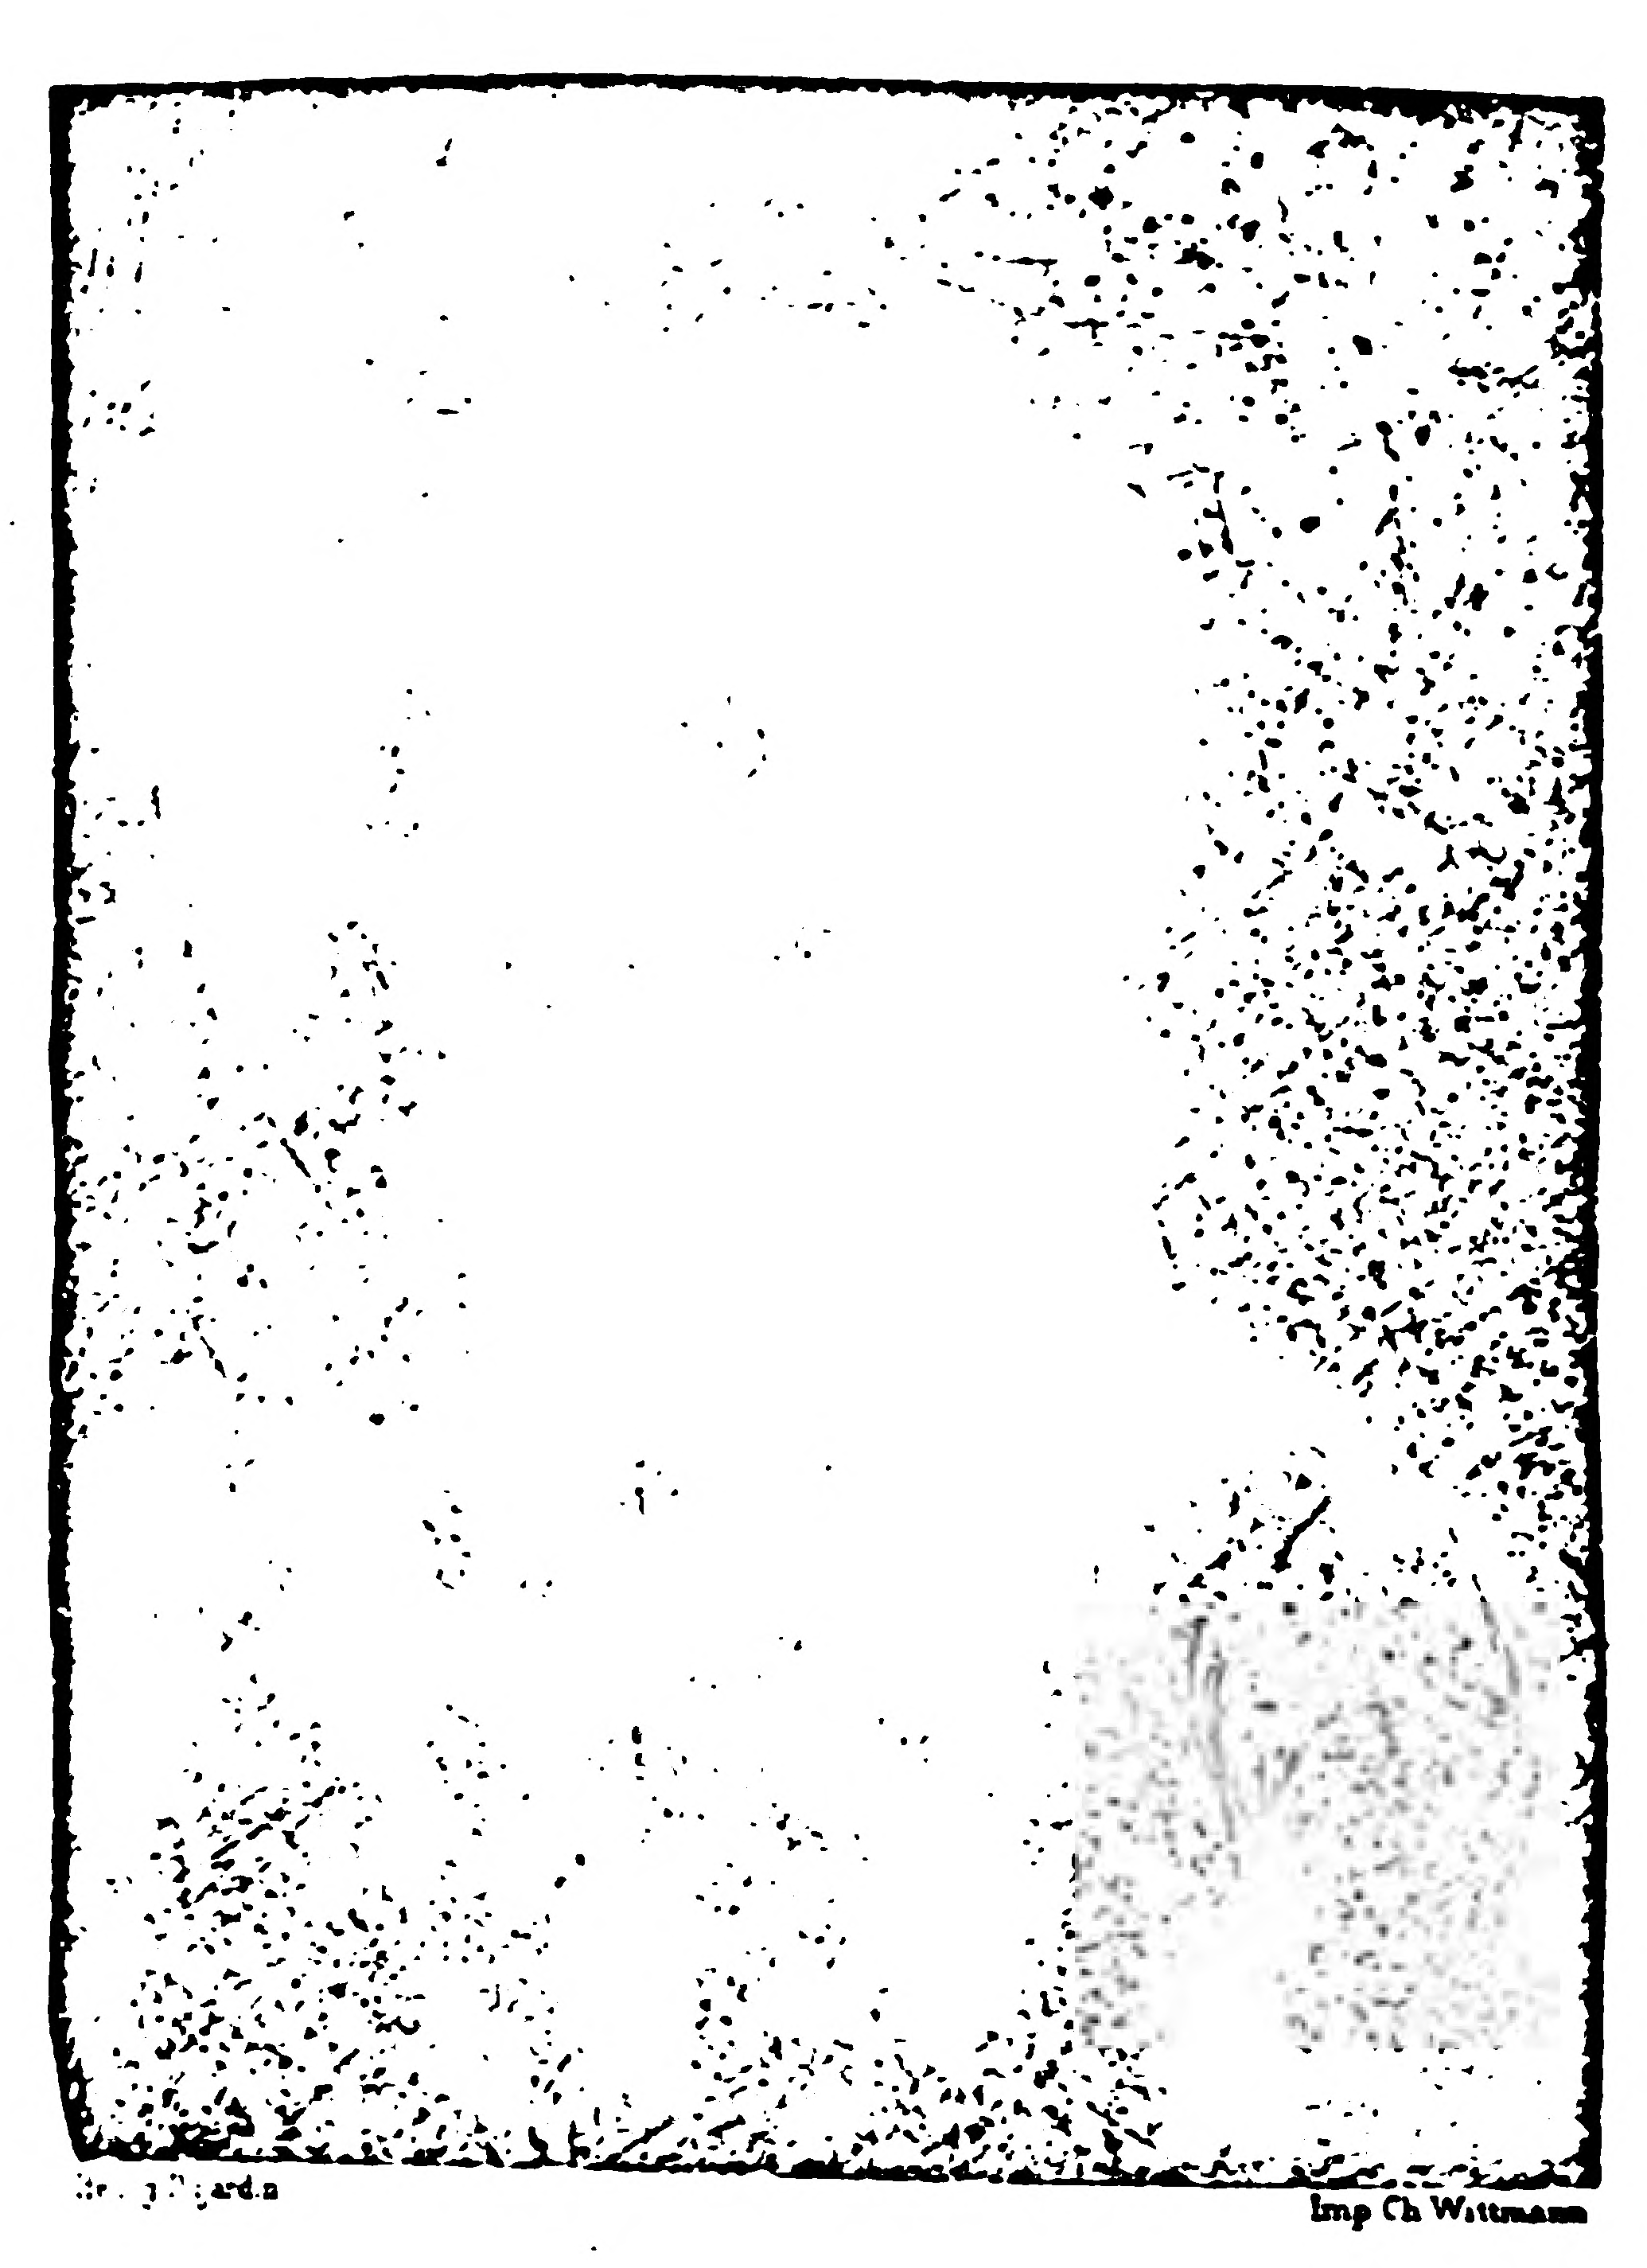
\includegraphics[height=0.61\textheight,keepaspectratio]{figures/PDF021_L0020_PORTRAIT_PLATE_DEGRADED.png}\par
  \vspace{1.0em}
  {\Large E. GALOIS\par}
  \end{center}
  \GalWitnessNote{W01-U002}{A second portrait image cannot yet be identified}{This separate scan page repeats the printed caption but contains a severely degraded portrait. The evidence does not show whether it is a second historical impression, a duplicate plate, or a duplication introduced during digitization, so it is preserved as a distinct page.}
  \GalSourcePageEnd
}

% PDF 022 / L0021 -- inspected blank topology.
\GalBlankTopologyPage{022}{L0021}{blank}{No historical letterpress or image.}
% PDF 023 / L0022 -- library stamps and shelfmark; intentionally not typeset.
\GalExcludedSourcePage{023}{L0022}{library_accession}{Harvard shelfmark and accession stamps.}

% Boundary protection: PDF 024 / L0023 begins INTRODUCTION. on printed folio v.
% It was inspected read-only for continuity and is not transcribed in W01.
